\documentclass{article}
\usepackage{graphicx} % Required for inserting images

\usepackage{amsmath}
\usepackage{amssymb}
\usepackage{float}
\usepackage[left=1.5cm, right=2cm, bottom=1in]{geometry}

\usepackage{subcaption}


\usepackage{subfiles}

\title{Composite games evolutionary dynamics in finite populations.}
\author{Henry Brooks}
\date{June - December 2025}

\begin{document}

\maketitle

\begin{abstract}
Final year masters project. Replicator dynamics in rock paper scissors (RPS) and composition of RPS and the snowdrift game (SD) in both the infinite and finite population cases. 
Payoff matrices and replicator derivations, stochastic simulations and drift analysis under different interaction process.
Extensive simulation tool for graphing and animation of the different processes and large ensemble averages for general games.
Derivation and analytical solution for observation
variable $H$ and exact calculation of critical population sizes under different parameters.
\end{abstract}


\section{Introduction}

\subsection{Background and Motivation}
% Introduce evolutionary game theory and its relevance.
% Contrast classical game theory with population-based dynamics.
% Motivate the importance of studying evolutionary dynamics.
Further the work on drift reversal (battle of the sexes, RPS).
Double drift reversal? Multiple games interacting. Falling in and out of 
stable RPS cyclic behaviour. 



\subsection{Deterministic and Stochastic Evolutionary Dynamics}
% Discuss limitations in finite populations.
% Motivate stochastic modelling approaches.
Infinite population replicator dynamics, stochastic equations for finite populations.

\subsection{Cyclic and Composite Games}
% Introduce Rock-Paper-Scissors as a canonical cyclic game.
% Motivate extensions to higher-dimensional and composite games.
RPS game, adding our 4th stategy.

This project focuses on a specific composite evolutionary game formed by 
combining a cyclic Rock-Paper-Scissors (RPS) subgame with a Snowdrift (SD) component.



\subsection{Aims of the project}
The aim of this project is to analyse evolutionary dynamics in finite populations 
for a specific composite game combining an RPS subgame with a Snowdrift component, 
focussing on the effects of stochastic drift, microscopic interaction processes, payoff parameters, and the effect of population size. This will involve the 
development of an efficient simulation and visualisation tool for analyzing symmetric games in finite populations.


\subsection{Objectives}
\begin{itemize}
    \item Formulate the composite RPS-SD game payoff structure and its deterministic replicator dynamics, including fixed points and stability.
    \item Implement efficient stochastic simulations of composite game (and general symmetric games) for differerent microscopic interaction processes (Moran, Local update, Fermi).
    \item Define an observation variable, $H$\cite{PhysRevLett.95.238701}, 
    for the game components, $H_{SD}, H_{RPS}, H_4$, and compute the expected drift $\langle \Delta H \rangle$ 
    both numerically from simulations and analytically.
    \item Analyse drift and trajectory behaviour across interaction processes,
     selection strengths, and payoff parameters.
    \item Calculate critical population sizes associated with drift
     reversal\cite{PhysRevLett.95.238701} under different conditions.
    \item Develop visualisation tools (time series and simplex-based plots)
     to compare stochastic and deterministic trajectories and analse drift.
\end{itemize}


\section{Literature Review}

\subsection{Evolutionary Game Theory}
% Overview of evolutionary game theory.
% Strategies as population fractions.
% Payoff matrices and fitness.

\subsection{Replicator Dynamics in Infinite Populations}
% Derivation of the replicator equation.
% Mean fitness and invariance properties.
% Fixed points and stability analysis.

\subsection{Rock-Paper-Scissors and Cyclic Dominance}
% Standard RPS dynamics.
% Neutral cycles and constants of motion.
% Biological and social examples of cyclic dominance.

\subsection{Finite Population Effects}
% Breakdown of deterministic dynamics at finite population sizes.
% Demographic noise and stochastic fluctuations.
% Absorbing states and fixation.

\subsection{Microscopic Interaction Processes}
% Overview of stochastic update rules.
% Markov processes and discrete state spaces.

\subsubsection{Moran Process}
% Definition and interpretation.
% Connection to replicator dynamics in the infinite-population limit.

\subsubsection{Local Update Process}
% Pairwise comparison dynamics.
% Differences from Moran selection.

\subsubsection{Fermi Process}
% Probabilistic imitation dynamics.
% Role of selection intensity.

\subsection{Drift and Observation Variables}
% Definition of stochastic drift.
% Observation variable H and expected change ΔH.
% Relation to stability and long-term behaviour.




\newpage
\section{Standard RPS}


The standard (general) rock paper scissors (RPS) payoff matrix is defined as:

\begin{align}
\begin{bmatrix}
    a & c & b\\
    b & a & c\\
    c & b & a
\end{bmatrix}
\end{align}

Let \( x \), \( y \), and \( z \) represent the fraction of players using rock, paper, and scissors respectively. Since \( z \) can be eliminated, we define:
\[
z = 1 - x - y
\]


Expected payoffs for each strategy can then be defined as follows:
\begin{align}
   \pi_R = a x + b \left(- x - y + 1\right) + c y \\
   \pi_P = a y + b x + c \left(- x - y + 1\right) \\
   \pi_S = a \left(- x - y + 1\right) + b y + c x
\end{align}


The replicator equations can be defined (ref Evo games and pop dynamics hofbauer) for $(x, y)$ using the standard formula:
\begin{equation}
    \dot x_i = x_i(\pi_i(x) - \langle \pi(x) \rangle)
\end{equation}

where the average payoff (or mean fitness) in the population is:
\[
\langle \pi(x) \rangle = x \pi_R + y \pi_P + z \pi_S
\]

This leads to the following replicator equations for x and y:

\begin{equation}
    \begin{split}
        \dot{x} &= x y \left(a x - a y - b x + b \left(-x - y + 1\right) + c y 
        - c \left(-x - y + 1\right)\right) \\
        & + x \left(-x - y + 1\right) \left(a x - a \left(-x - y + 1\right)
        - b y + b \left(-x - y + 1\right) - c x + c y\right)
    \end{split}
\end{equation}

\begin{equation}
    \begin{split}
        \dot{y} &= x y \left(- a x + a y + b x - b \left(- x - y + 1\right) - c y 
        + c \left(- x - y + 1\right)\right) \\
        & + y \left(- x - y + 1\right) \left(a y - a \left(- x - y + 1\right)
        + b x - b y - c x + c \left(- x - y + 1\right)\right)
    \end{split}
\end{equation}


Defining $F = \dot x, G = \dot y$, the following derivatives form the Jacobian used to determine the stability of the system:
\begin{align}
    \frac{dF}{dx} &= x y (a - 2b + c) 
    + x (2a - b - c)(-x - y + 1) \nonumber \\
    &\quad - x \left(a x - a(-x - y + 1) - b y + b(-x - y + 1) - c x + c y\right) \nonumber \\
    &\quad + y \left(a x - a y - b x + b(-x - y + 1) + c y - c(-x - y + 1)\right) \nonumber \\
    &\quad + (-x - y + 1) \left(a x - a(-x - y + 1) - b y + b(-x - y + 1) - c x + c y\right) \\
    \frac{dF}{dy} &= x y (-a - b + 2c) 
    + x (a - 2b + c)(-x - y + 1) \nonumber \\
    &\quad + x \left(a x - a y - b x + b(-x - y + 1) + c y - c(-x - y + 1)\right) \nonumber \\
    &\quad - x \left(a x - a(-x - y + 1) - b y + b(-x - y + 1) - c x + c y\right) \\
    \frac{dG}{dx} &= x y (-a + 2b - c)
    + y (a + b - 2c)(-x -y + 1) \nonumber \\
    &\quad +y (-ax + ay + bx - b (-x -y + 1) - cy + c (-x-y+1)) \nonumber \\
    &\quad -y (ay - a(-x-y+1) + bx - by - cx + c(-x-y+1)) \\
    \frac{dG}{dy} &= x y (a + b - 2c)
    + x \left( -a x + a y + b x - b(-x - y + 1) - c y + c(-x - y + 1) \right) \nonumber \\
    &\quad + y (2a - b - c)(-x - y + 1) \nonumber \\
    &\quad - y \left( a y - a(-x - y + 1) + b x - b y - c x + c(-x - y + 1) \right) \nonumber \\
    &\quad + (-x - y + 1) \left( a y - a(-x - y + 1) + b x - b y - c x + c(-x - y + 1) \right)
\end{align}


The Jacobian is as follows:
\[
J = 
\begin{bmatrix}
\frac{\partial F}{\partial x} & \frac{\partial F}{\partial y} \\
\frac{\partial G}{\partial x} & \frac{\partial G}{\partial y}
\end{bmatrix}
\]


Eigenvalues at the standard RPS game (a = 0, b = 1, c = -1):
\[
\left\{
    -\frac{1}{2} \sqrt{16 x^{2} + 16 x y - 16 x + 16 y^{2} - 16 y + 4} \,, \quad
    \frac{1}{2} \sqrt{16 x^{2} + 16 x y - 16 x + 16 y^{2} - 16 y + 4}
\right\}
\]

At the internal fixed point of $(x,y) = (\frac{1}{3}, \frac{1}{3})$, 
$\lambda_{1,2} =\left\{- \frac{\sqrt{3}}{3} i, \frac{\sqrt{3}}{3} i\right\}$

\par
No real parts of any eigenvalues, and imaginary components exist therefore neutral stability in standard RPS.






\section{Augmented RPS}


The augmented game can be described by the following payoff matrix.

\begin{align}
\label{AugRpsMatrix}
\begin{bmatrix}
    a & c & b & \gamma\\
    b & a & c & \gamma\\
    c & b & a & \gamma\\
    a + \beta & a + \beta & a + \beta & 0
\end{bmatrix}
\end{align}

\begin{align} \nonumber
\label{CompositeGame}
\begin{bmatrix}
    \langle RPS \rangle & \gamma\\
    \beta & 0 \\
\end{bmatrix}
\end{align}

Where the strategies are labelled as R,P,S (as before) and L (the loner strategy).
From this the Jacobian matrix can be derived with dimensions $3 \times 3$ after using the trick to remove one replicator equation. (q = 1 - x - y - z)

\subsection{Payoffs}
Payoffs for the augmented game:
\begin{align}
    \pi_R &= a x + b z + c y + \gamma (- x - y - z + 1)\\
    \pi_P &= a y + b x + c z + \gamma (- x - y - z +1) \\
    \pi_S &= a z + b y + c x + \gamma (- x - y - z + 1)\\
    \pi_L &= x (a + \beta) + y (a + \beta) + z (a + \beta)
\end{align}

\subsection{Replicator equations}

\begin{align} 
    \dot x &= x (a x + b z + c y + \gamma (- x - y - z + 1) - x (a x + b z + c y + \gamma (- x - y - z + 1)) \nonumber \\
    &- y (a y + b x + c z + \gamma (- x - y - z + 1)) - z (a z + b y + c x + \gamma (- x - y - z + 1)) \nonumber \\
    &- (x (a + \beta) + y (a + \beta) + z (a + \beta)) (- x - y - z + 1))
\end{align}

\begin{align}
\dot{y} &= y \big(a y + b x + c z + \gamma (-x - y - z + 1)
- x (a x + b z + c y + \gamma (-x - y - z + 1)) \nonumber \\
&\quad - y (a y + b x + c z + \gamma (-x - y - z + 1))
- z (a z + b y + c x + \gamma (-x - y - z + 1)) \nonumber \\
&\quad - (x (a + \beta) + y (a + \beta) + z (a + \beta)) (-x - y - z + 1) \big)
\end{align}


\begin{align}
\dot{z} &= z \big(a z + b y + c x + \gamma (-x - y - z + 1)
- x (a x + b z + c y + \gamma (-x - y - z + 1)) \nonumber \\
&\quad - y (a y + b x + c z + \gamma (-x - y - z + 1))
- z (a z + b y + c x + \gamma (-x - y - z + 1)) \nonumber \\
&\quad - (x (a + \beta) + y (a + \beta) + z (a + \beta)) (-x - y - z + 1) \big)
\end{align}

\noindent
Reduced the dimensions to just 3 replicator equations in x, y and z as q = 1 - x - y - z. \\
Jacobian formed as before, $F = \dot{x}, G = \dot{y}, P = \dot{z}$
\[
J = 
\begin{bmatrix}
\frac{\partial F}{\partial x} & \frac{\partial F}{\partial y} &\frac{\partial F}{\partial z} \\[6pt]
\frac{\partial G}{\partial x} & \frac{\partial G}{\partial y} &\frac{\partial G}{\partial z} \\[6pt]
\frac{\partial P}{\partial x} & \frac{\partial P}{\partial y} & \frac{\partial P}{\partial z}
\end{bmatrix}
\]



\subsection{Stability}

Eigenvalues computed using Sympy python library, simplified by hand - floating point precision issue starting to come into play but values are clear (0, 2/9, -2/3 etc).


\par
With a = 0, b = 1, c = -1, $\gamma = 0.2, \beta = 0.1$ we have an internal fixed point at $(2/9, 2/9,2/9, 1/3)$ (see matrix \ref{AugRpsA}) with eigenvalues (Re, Im):
\begin{equation}
    \left\{
    ( 0, \  0.222222222222222 \sqrt{3}),
    ( -0.0666666666666667, \  0),
    ( 0, \  - 0.222222222222222 \sqrt{3})
    \right\}
\end{equation}

\par
All the real parts are $<=0$, indicating neutral stability (oscillations at fixed distance around the interior fixed point) also visible in the simulations \ref{fig:3d}.

\par    
See figure \ref{fig:3d} for the 4 simplex plot of these dynamics for the local update and Moran processes aswell as numerical solution of the replicator system of ODE's derived from the standard replicator equation (local update in the limit $N \to \infty$). With a suitably large population the local and Moran processes are following the deterministic trajectory but with added noise.



\begin{figure}[h]
    \centering
    \includegraphics[width=1\linewidth]{images/3d.png}
    \caption{N=1000, iterations=1,000,000}\label{fig:3d}
\end{figure}

\section{Interaction processes \ simulations}
\subsection{Moran}

\begin{figure}[h]
    \centering
    \includegraphics[width=0.7\linewidth]{images/moran_time_series.png}
    \caption{population size 60000 Moran process, along with numerical solution to adjusted dynamics.}
    \label{fig:placeholder}
\end{figure}


\subsection{Local update}

\begin{figure}[h]
    \centering
    \includegraphics[width=0.7\linewidth]{images/lu_timeseries.png}
    \caption{Time series of local update with population 20000, simulation trajectory normalized, compared with the numerical solution of the replicator equations derived from FP equation \cite{PhysRevLett.95.238701}}
    \label{fig:placeholder}
\end{figure}


\subsection{Fermi process}

\subsection{Link to deterministic equations $\lim_{N\to\infty}$}
Adjusted deterministic equations for the interaction processes, derived from the fokker planck expansions of the interaction processes defined (master equation).



\subsection{Transition probabilities}

Finite population, $i$ rock players, $j$ paper players, $k$ scissors players, and $N - i - j - k$ $+$ players. In the Moran process an individual is chosen proportionally to their fitness in the population, therefore we need the global average fitness $\langle \pi \rangle$, the average payoff is $\langle \pi \rangle = \frac{i}{N} \pi_R + \frac{j}{N} \pi_P + \frac{k}{N} \pi_S + \frac{N - i - j -k}{N} \pi_+$

For the Moran process the transition probabilities are as follows:
\begin{equation}
    T^{R \rightarrow +} = \frac{1}{2} \frac{1 - w + w \pi_+}{1 - w + w \langle \pi \rangle} \frac{i}{N} \frac{N - i - j - k}{N}
\end{equation}  
\begin{equation}
    T^{+ \rightarrow R} = \frac{1}{2} \frac{1 - w + w \pi_R}{1 - w + w \langle \pi \rangle} \frac{i}{N} \frac{N - i - j - k}{N}
\end{equation}  

Also transitions within RPS

\begin{equation}
    T^{R \rightarrow S} = \frac{1}{2} \frac{1 - w + w \pi_S}{1 - w + w \langle \pi \rangle} \frac{i}{N} \frac{k}{N}
\end{equation}  

\begin{equation}
    T^{S \rightarrow R} = \frac{1}{2} \frac{1 - w + w \pi_R}{1 - w + w \langle \pi \rangle} \frac{i}{N} \frac{k}{N}
\end{equation}  

\par
The rest of the transitions, $T^{R \rightarrow P}, T^{P \rightarrow R}, T^{S \rightarrow P}, T^{P \rightarrow S}, T^{P \rightarrow +}, T^{+ \rightarrow P}, T^{ S \rightarrow +}, T^{+ \rightarrow S}$
formed from permuations ($R, P, S, +$) and ($i, j, k, N-i-j-k$) \\

\par
For the local update process we compare payoffs between only 2 randomly selected individuals $a$ and $b$.


\begin{equation}
  T^{R \rightarrow +} = \left (\frac{1}{2} + \frac{w}{2} \frac{\pi_+ - \pi_R}{\Delta \pi_{\text{max}}} \right ) \frac{i}{N} \frac{N - i - j - k}{N}
\end{equation}


Can simply define these transitions as:
\begin{equation}
  \phi(b \rightarrow a) \frac{N_a N_b}{N^2}
\end{equation}
Given an appropriate $\phi$ reproductive function.


\subsubsection{Master equation}


\subfile{fokker_planck_derivation.tex}

\newpage
\subsection{Constant of motion $\Delta H$ definition (drift)}
\subfile{delta_H_derivation.tex}





\newpage
\section{Drift}





\begin{align} \label{AugRpsA}
\begin{bmatrix}
    0 & -s & 1 & 0.2\\
    1 & 0 & -s & 0.2\\
    -s & 1 & 0 & 0.2\\
    0.1 & 0.1 & 0.1 & 0
\end{bmatrix}
\end{align}


\begin{figure}[h]
    \centering
    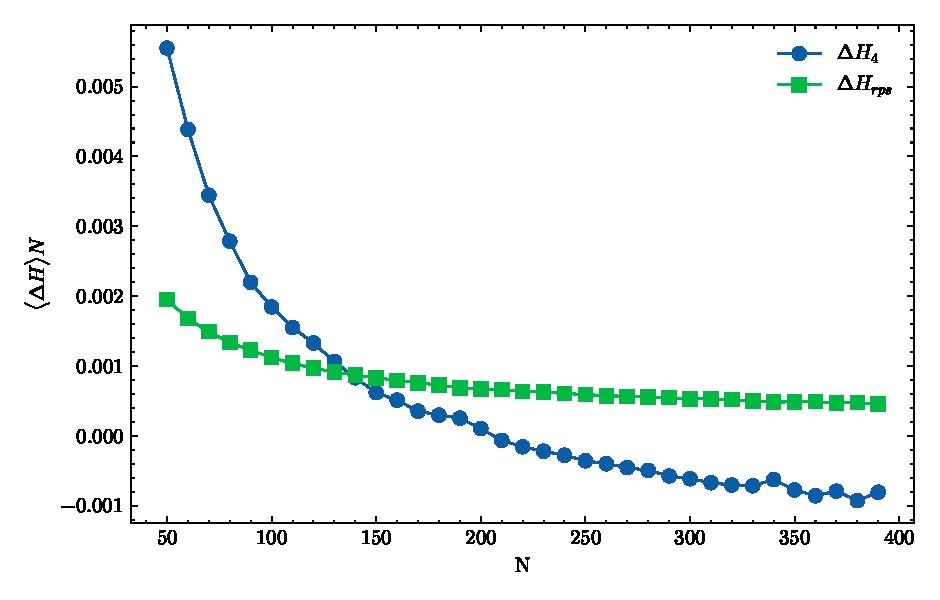
\includegraphics[width=0.6\linewidth]{images/moran_reversal.eps}
    \caption{Drift reversal in the above game \ref{AugRpsA}, in the 4th strategy $\langle \Delta H \rangle$ changes sign. Averages over 10,000,000 realisations, fixed $w=0.45$, $\Delta H_{rps}$ approaches 0 but does not reverse, $s=1$}
    \label{fig:drift_reversal_1}
\end{figure}

\begin{figure}[h]
    \centering
    \includegraphics[width=0.6\linewidth]{images/drift_reversal_rps.png}
    \caption{Drift reversal in the standard RPS game - 0 playing 4th strategy, $s=0.8$, deterministic case the internal fixed point is stable ($\langle \Delta H_{rps}\rangle>0$) but again it changes sign at a small population size, average over 10,000,000 realisations. Change of sign at $N\approx470$}
    \label{fig:drift_standard_rps}
\end{figure}


\begin{figure}
    \centering
    \includegraphics[width=0.6\linewidth]{images/drift_4.eps}
    \caption{Moran and local update drift for $\Delta H_4$ - $2 \times 10^7$ realizations , needs more average but drift reversal by N = 400, with w = 0.45}
    \label{fig:placeholder}
\end{figure}


\begin{figure}[h]
    \centering
    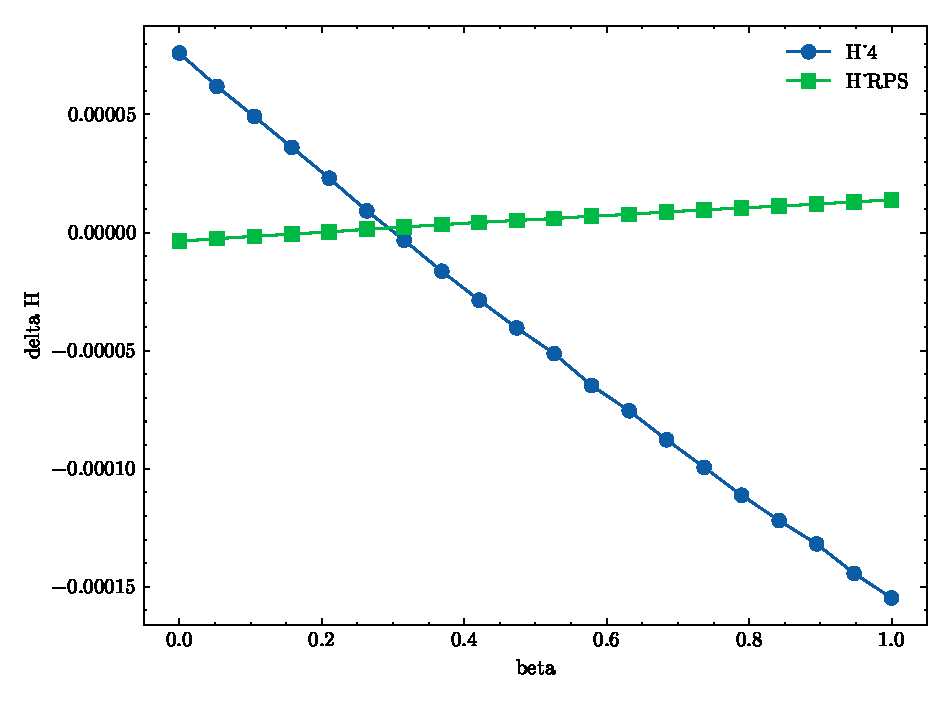
\includegraphics[width=0.5\linewidth]{parameter_tests/beta_test.eps}
    \caption{$\langle \Delta H_4 \rangle$ and $\langle \Delta H_{rps}\rangle$ for range of $\beta$ values (0 to 1) in above matrix, fixed value of $\gamma = 0.5, w = 0.45, N=200$}
\end{figure}

\begin{align}
\begin{bmatrix}
    0 & -s & 1 & 0.5\\
    1 & 0 & -s & 0.5\\
    -s & 1 & 0 & 0.5\\
    0 + \beta & 0 + \beta & 0 + \beta & 0
\end{bmatrix}
\end{align}

\begin{align}
\begin{bmatrix}
    0 & -s & 1 & \gamma\\
    1 & 0 & -s & \gamma\\
    -s & 1 & 0 & \gamma\\
    0 + \beta & 0 + \beta & 0 + \beta & 0
\end{bmatrix}
\end{align}

\begin{figure}[h]
    \centering
    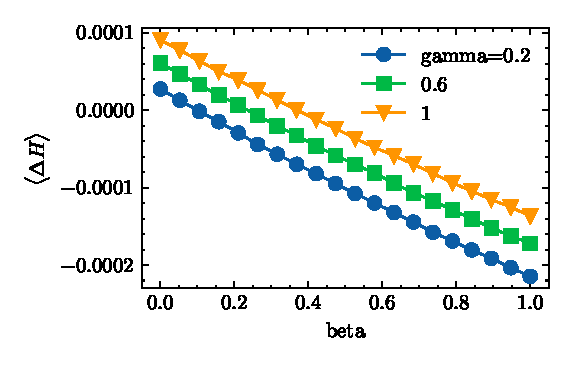
\includegraphics[width=0.6\linewidth]{parameter_tests/fixed_n_gamma_beta.eps}
    \caption{$\langle\Delta H_4\rangle$ for different $\beta$, for 3 different $\gamma$}
    \label{fig:placeholder}
\end{figure}

\begin{figure}[h]
    \centering
    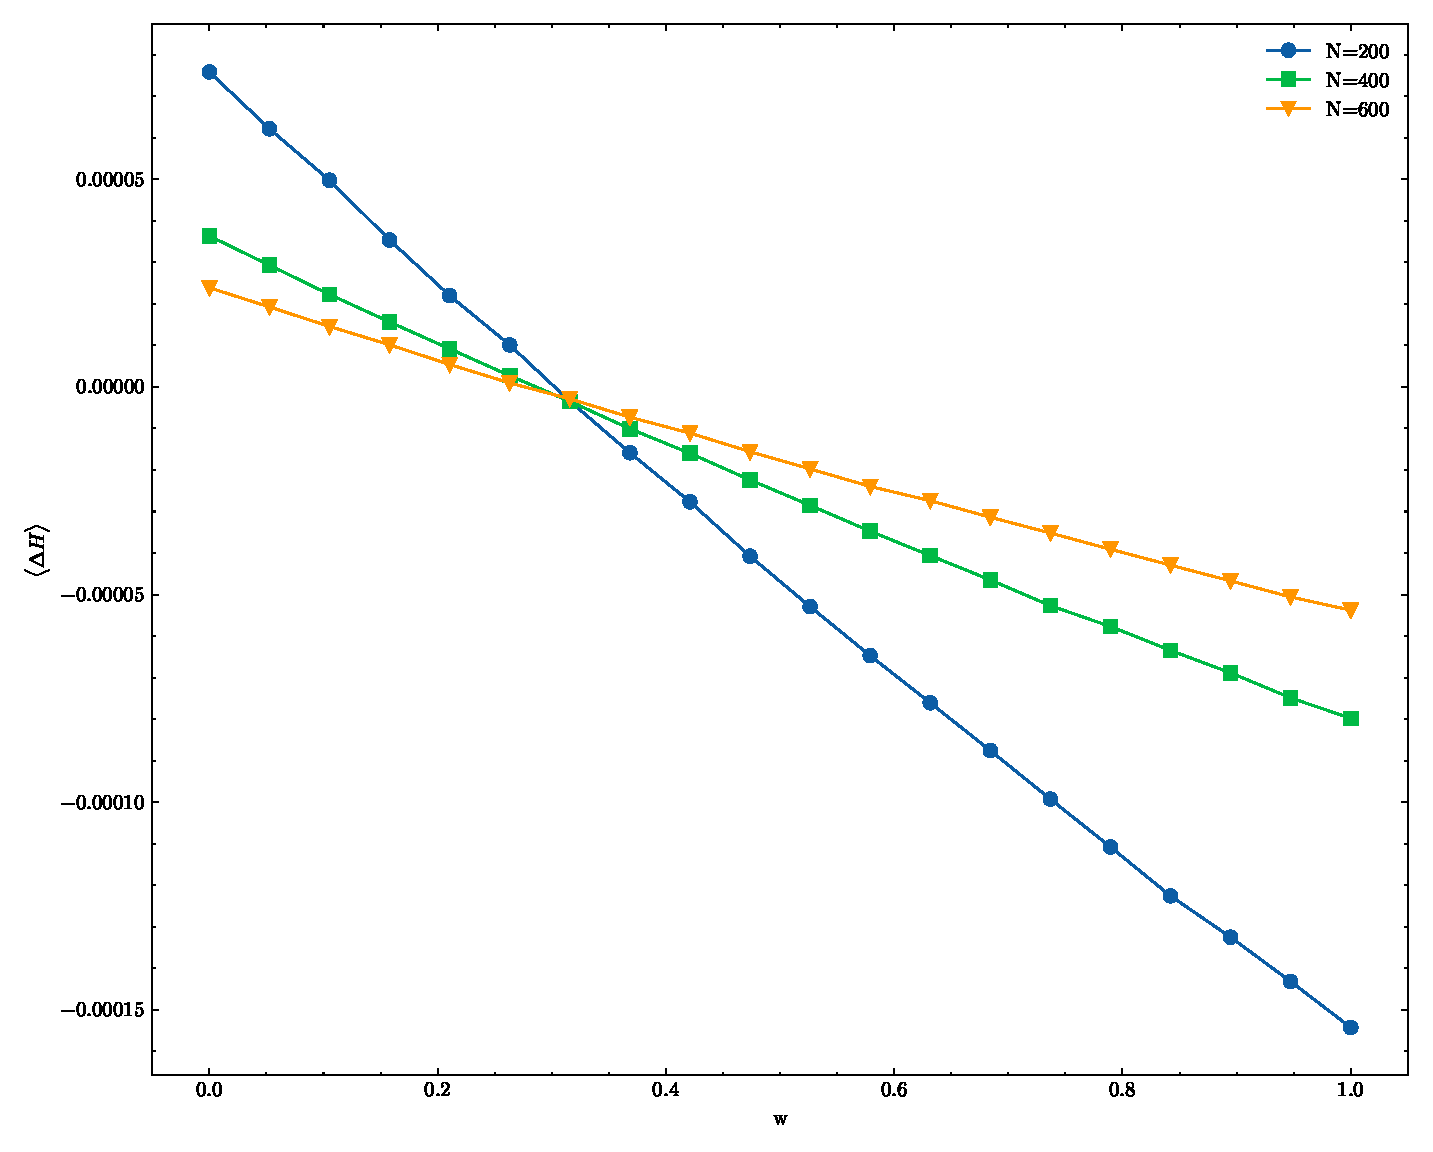
\includegraphics[width=0.6\linewidth]{parameter_tests/fixed_gamma_parameter.eps}
    \caption{$\langle\Delta H_4\rangle$ for different $\beta$ at different pop sizes.}
    \label{fig:placeholder}
\end{figure}







\clearpage
\newpage
\subsection{Critical population size $N_c$}

\par
The critical population size where drift occurs for a varying selection pressure w.
\\
Implemented using the previous simulation code at suitably large simulation repetitions, binary search around the change of sign for the $\Delta H_4$ value and repeated for range of $w$'s.

\begin{figure}[h]
    \centering
    \includegraphics[width=0.6\linewidth]{images/critN.png}
    \caption{Critical N against W, need to average this with more realizations.}
    \label{fig:placeholder}
\end{figure}

\begin{figure}[h]
    \centering
    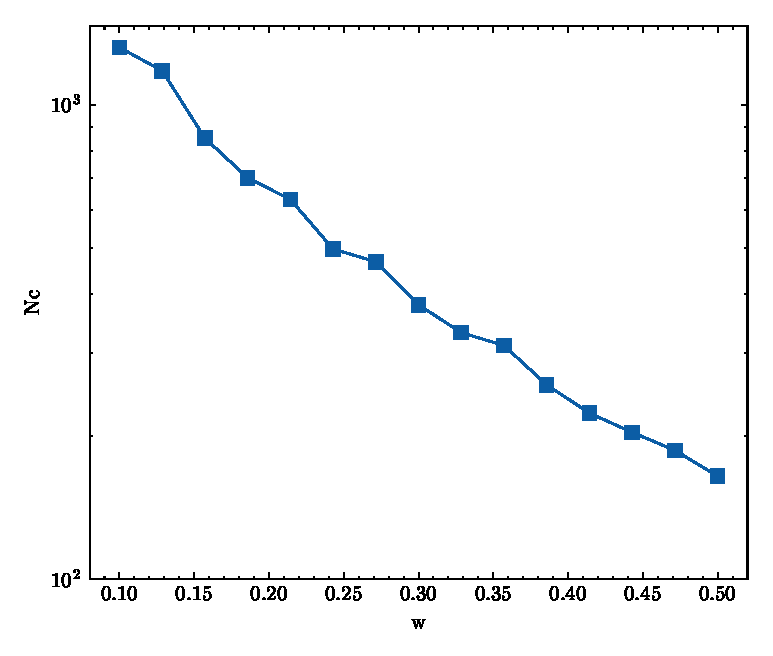
\includegraphics[width=0.5\linewidth]{images/w_test.eps}
    \caption{$5 \times 10^{7}$ realizations, critical N for drift reversal in \ref{AugRpsA}}
    \label{fig:placeholder}
\end{figure}





\begin{figure}[h]
    \centering
    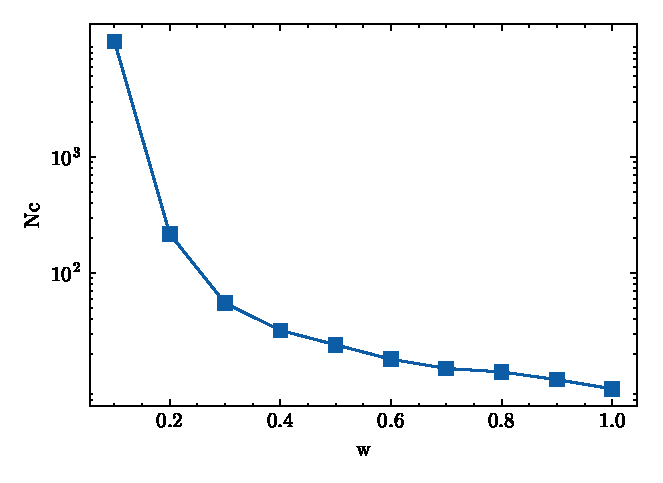
\includegraphics[width=0.5\linewidth]{parameter_tests/crit_n_beta.eps}
    \caption{Critical population size $N_c$ for range of $\beta$ from 0 to 1, fixed $w=0.45$, fixed $\gamma=0.5$}
    \label{fig:placeholder}
\end{figure}

\begin{figure}[h]
    \centering
    \includegraphics[width=0.5\linewidth]{parameter_tests/crit_n_gamma.eps}
    \caption{Critical population size $N_c$ for range of $\gamma$ from 0 to 1, fixed $w=0.45$, fixed $\beta=0.2$}
    \label{fig:placeholder}
\end{figure}
x axis label incorrect below


\clearpage



\begin{figure}
\begin{subfigure}{.3\textwidth}
  \centering
  \includegraphics[width=1\linewidth]{images/initial_cloud.png}
  \caption{Initial}
  \label{fig:sfig1}
\end{subfigure}%
\begin{subfigure}{.3\textwidth}
  \centering
  \includegraphics[width=1\linewidth]{images/point_cloud_2.png}
  \caption{N = 200, rps drift outwards}
  \label{fig:sfig1}
\end{subfigure}%
\begin{subfigure}{.3\textwidth}
  \centering
  \includegraphics[width=1\linewidth]{images/point_cloud_3.png}
  \caption{N = 100, rps drift out and strategy 4 drift down}
  \label{fig:sfig2}
\end{subfigure}
\label{fig:fig}
\caption{Initial random starting points, at low population we seee RPS drift occuring first, and the game is still at SD equilibrium, but at lower strategy e.g $N< 150$ as in the drift graph further up we seee reversal of both strategies to the bottom 3 corners, when $c > b$, or to all 4 corners when $b = c$ ($b = \beta, c = \gamma$ in the matrices in the document), similar results for both $s=1, s=0.8$ in the small population cases and both time RPS drifst out before SD and SD drifts at low population - only difference in large population case}
\end{figure}

\begin{figure}
    \centering
    \includegraphics[width=0.4\linewidth]{images/point_cloud_4.png}
    \caption{Large pop - fixes in orbit about center, s = 1 - very large population for neutrally stable RPS}
\end{figure}

\begin{figure}
    \centering
    \includegraphics[width=0.5\linewidth]{images/point_cloud_5.png}
    \caption{large pop, s = 0.8, converges to central fixed point. - large population for asymptotically stable RPS - $s < 1$}
\end{figure}

\begin{figure}
    \centering
    \includegraphics[width=0.5\linewidth]{images/50000POP.png}
    \caption{large pop, matrix in diagram}
\end{figure}

\begin{figure}
\begin{subfigure}{.5\textwidth}
  \centering
  \includegraphics[width=1\linewidth]{images/50000POP.png}
  \caption{$N = 50000$}
\end{subfigure}%
\begin{subfigure}{.5\textwidth}
  \centering
  \includegraphics[width=1\linewidth]{images/850POP.png}
  \caption{$N = 850$}
\end{subfigure}%
\caption{$w=0.45$, Strong attracting RPS with matrix in figure, reversal seen in SD but not in RPS, large population size tends to the deterministic case. - generate a $\Delta H_4, \Delta H_{RPS}$ plot for the above to show the drift reversal in SD game and not in RPS.}
\end{figure}



\begin{figure}[h]
    \centering
    \includegraphics[width=1\linewidth]{images/RPS_cross_fist.png}
    \caption{Same game used for above cloud - RPS crossing the x axis at a lower $N_c$ - explains SD drift first}
\end{figure}


\clearpage
\section{Refs}
Scienceplots library for simple styling ref. \cite{SciencePlots} 

\noindent
Numba jit python compiler - used for large optimisations pre compiling intensive functions to fast machine code. \cite{lam2015numba} Huge performance increase using numba in no-python mode compiling all the critical simulation methods into machine code and inlining them where appropriate to reduce function call overhead. Reached feasible simulation speed.

\noindent
Drift reversal paper \cite{PhysRevLett.95.238701}


\bibliographystyle{plain}
\bibliography{ref}
\end{document}
